\documentclass{article}

\usepackage[a-2u]{pdfx}
\usepackage[utf8]{inputenc}
\usepackage{array}
\usepackage[ddmmyyyy]{datetime}
\usepackage{geometry}
\usepackage{hyperref}
\usepackage{listings}
\usepackage{xcolor}
\usepackage{graphicx}
\usepackage{float}

\renewcommand{\dateseparator}{.}
\renewcommand{\baselinestretch}{1.5}

\geometry{margin=2cm}

\def\ResearchProject{Research project}
\def\CompanyProject{Company project}
\def\SoftwareProject{Software project}

% METADATA SECTION START
\def\StudentsFullName{Martin Čorovčák}
\def\StudyProgram{Computer Science --- Software and Data Engineering}
\def\ProjectTitle{LLM Advisor for Migration Between ORM/ODM/OGM Frameworks}
\def\ProjectType{\ResearchProject}
\def\SupervisorFullName{Ing. Pavel Koupil, Ph.D.}
\def\ConsultantsFullName{doc. RNDr. Irena Holubová, Ph.D.}
% METADATA SECTION END

\title{\ProjectTitle}
\author{\StudentsFullName}

\begin{document}

\centerline{\Large \textbf{Specification of team software project}}
\centerline{ \textbf{Department of Software Engineering}}
\centerline{ \textbf{Faculty of Mathematics and Physics, Charles University}}
\bigskip
{\noindent\begin{tabular*}{\textwidth}{ >{\raggedleft}m{4cm} l}
\textbf{Solvers:} & \StudentsFullName \\
\textbf{Study program:} & \StudyProgram \\[1em]
\textbf{Project title:} & \ProjectTitle \\
\textbf{Project type:} & \ProjectType \\[1em]
\textbf{Supervisor:} & \SupervisorFullName \\ 
\textbf{Consultants:} & \ConsultantsFullName \\
\end{tabular*}}

\section{Introduction}
Within the Adaptive Data Management (ADaM) Research Group at the Department of Software Engineering, Charles University, extensive research has been conducted on the unified management of multi-model data. This line of work has addressed several core aspects of heterogeneous data processing, including conceptual modeling, querying, evolution, and optimization across diverse database paradigms. As part of these efforts, earlier work by Milan Abrahám~\cite{ormorpherthesis} introduced the \textit{ORMorpher} tool, a rule-based system for translating and optimizing schemas and queries between .NET Object-Relational Mapping frameworks, namely Entity Framework Core\footnote{\url{https://learn.microsoft.com/en-us/ef/core/}}, NHibernate\footnote{\url{https://nhibernate.info/}}, and Dapper\footnote{\url{https://github.com/DapperLib/Dapper}}, using a unified intermediate representation. This line of research was subsequently formalized in a joint publication~\cite{ase2025}, which describes the parser-builder architecture and the ILP-based framework-selection advisor underlying ORMorpher.

The objective of this project is to significantly extend the scope of ORMorpher within the broader \emph{Universal Object Mapping (UOM)} project~\cite{uomrepo}. In particular, the project targets cross-paradigm translation from .NET ORM frameworks to Java-based Object-Document Mapping frameworks, represented by Spring Data MongoDB\footnote{\url{https://docs.spring.io/spring-data/mongodb/reference/}}, and Object-Graph Mapping frameworks, represented by Spring Data Neo4j\footnote{\url{https://docs.spring.io/spring-data/neo4j/reference/}}. Rather than relying primarily on a heuristic rule engine, the project explores an LLM-driven iterative translation pipeline intended to support more flexible and semantically informed migration between heterogeneous framework ecosystems.

To achieve this, the project introduces the \textbf{LLM Advisor} as its main architectural contribution. The proposed solution is based on a semi-deterministic, graph-structured workflow built using the open-source LangChain LangGraph framework\footnote{\url{https://www.langchain.com/langgraph}}. Within this workflow, autonomous reasoning-and-acting (ReAct) agents are orchestrated to iteratively generate, validate, and refine translation outputs. The process combines multiple forms of contextual information and external tooling, including database schemas, retrieval of relevant and up-to-date framework documentation, and compilation or validation against sandboxed backend services. In this way, the project aims to provide an intelligent translation advisor capable of addressing forms of structural and semantic heterogeneity that are too substantial to be handled robustly by deterministic rule-based translators alone.

\subsection{Relation to other projects}

This project builds directly on the \emph{ORMorpher} project~\cite{ormorpherthesis,ormorpherrepo}, which features a .NET Roslyn compiler-based translations from .NET ORM to Abstract Representation and vice-versa using heuristics and schema/query string parsers (see Figure~\ref{fig:ormorpher-architecture}), then ILP Advisor (benchmarking, optimization and subsequent framework selection), and lastly ASP.NET backend with Angular frontend (see Figure~\ref{fig:ormorpher-ui}). The future \textbf{LLM Advisor} can be integrated into ORMorpher's existing UI as a plugin widget, but also acts as a separate standalone service with its own REST API, allowing for future reuse in other contexts (e.g., publicly available MCP server\footnote{\url{https://modelcontextprotocol.io/docs/getting-started/intro}, \url{https://mcpservers.org/}}, MM-cat schema translations~\cite{mmcat}).

\begin{figure}[ht]
  \centering
  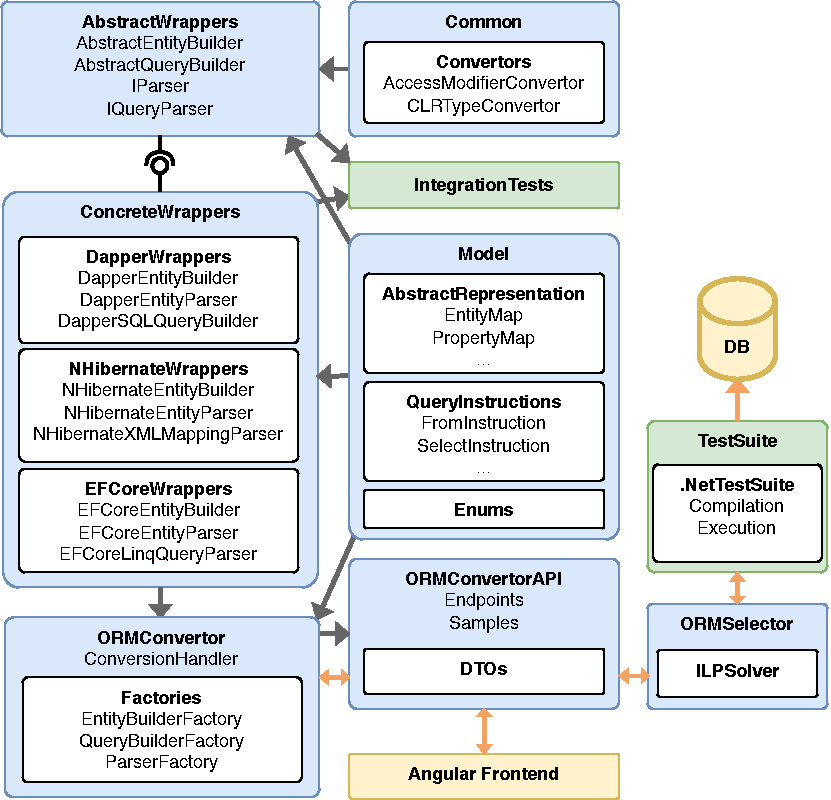
\includegraphics[width=0.55\textwidth]{img/ormorpher-architecture.pdf}
  \caption{ORMorpher architecture diagram. Extracted from ORMorpher thesis~\cite{ormorpherthesis}.}
  \label{fig:ormorpher-architecture}
\end{figure}

\begin{figure}[ht]
  \centering
  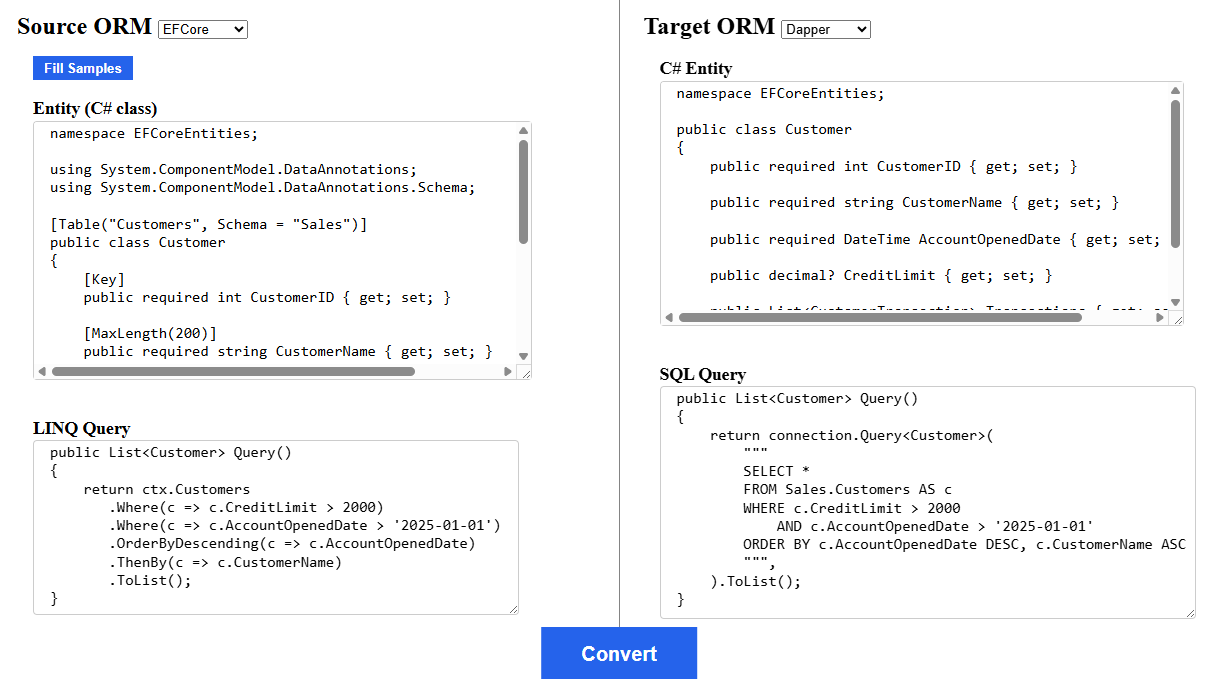
\includegraphics[width=0.8\textwidth]{img/ormorpher-ui.png}
  \caption{ORMorpher UI. Lives on \url{http://116.203.208.55/orm/home}. Extracted from ORMorpher thesis~\cite{ormorpherthesis}.}
  \label{fig:ormorpher-ui}
\end{figure}

\section{Project Description}

The main goal is to design and implement an \emph{LLM-driven translation pipeline} that accepts a source ORM schema (i.e. from EFCore, NHibernate, and Dapper) and a set of associated queries for one framework and produces equivalent schemas and queries for one or more target frameworks. The complete \emph{UOM} system includes database setup, defining and automating ETL processes, setup scripts, and providing a user-friendly interface for managing the translation process. Then, the advisor pipeline handles translation, iterative validation/error correction, and results presentation.


\begin{figure}[htbp]
\centering
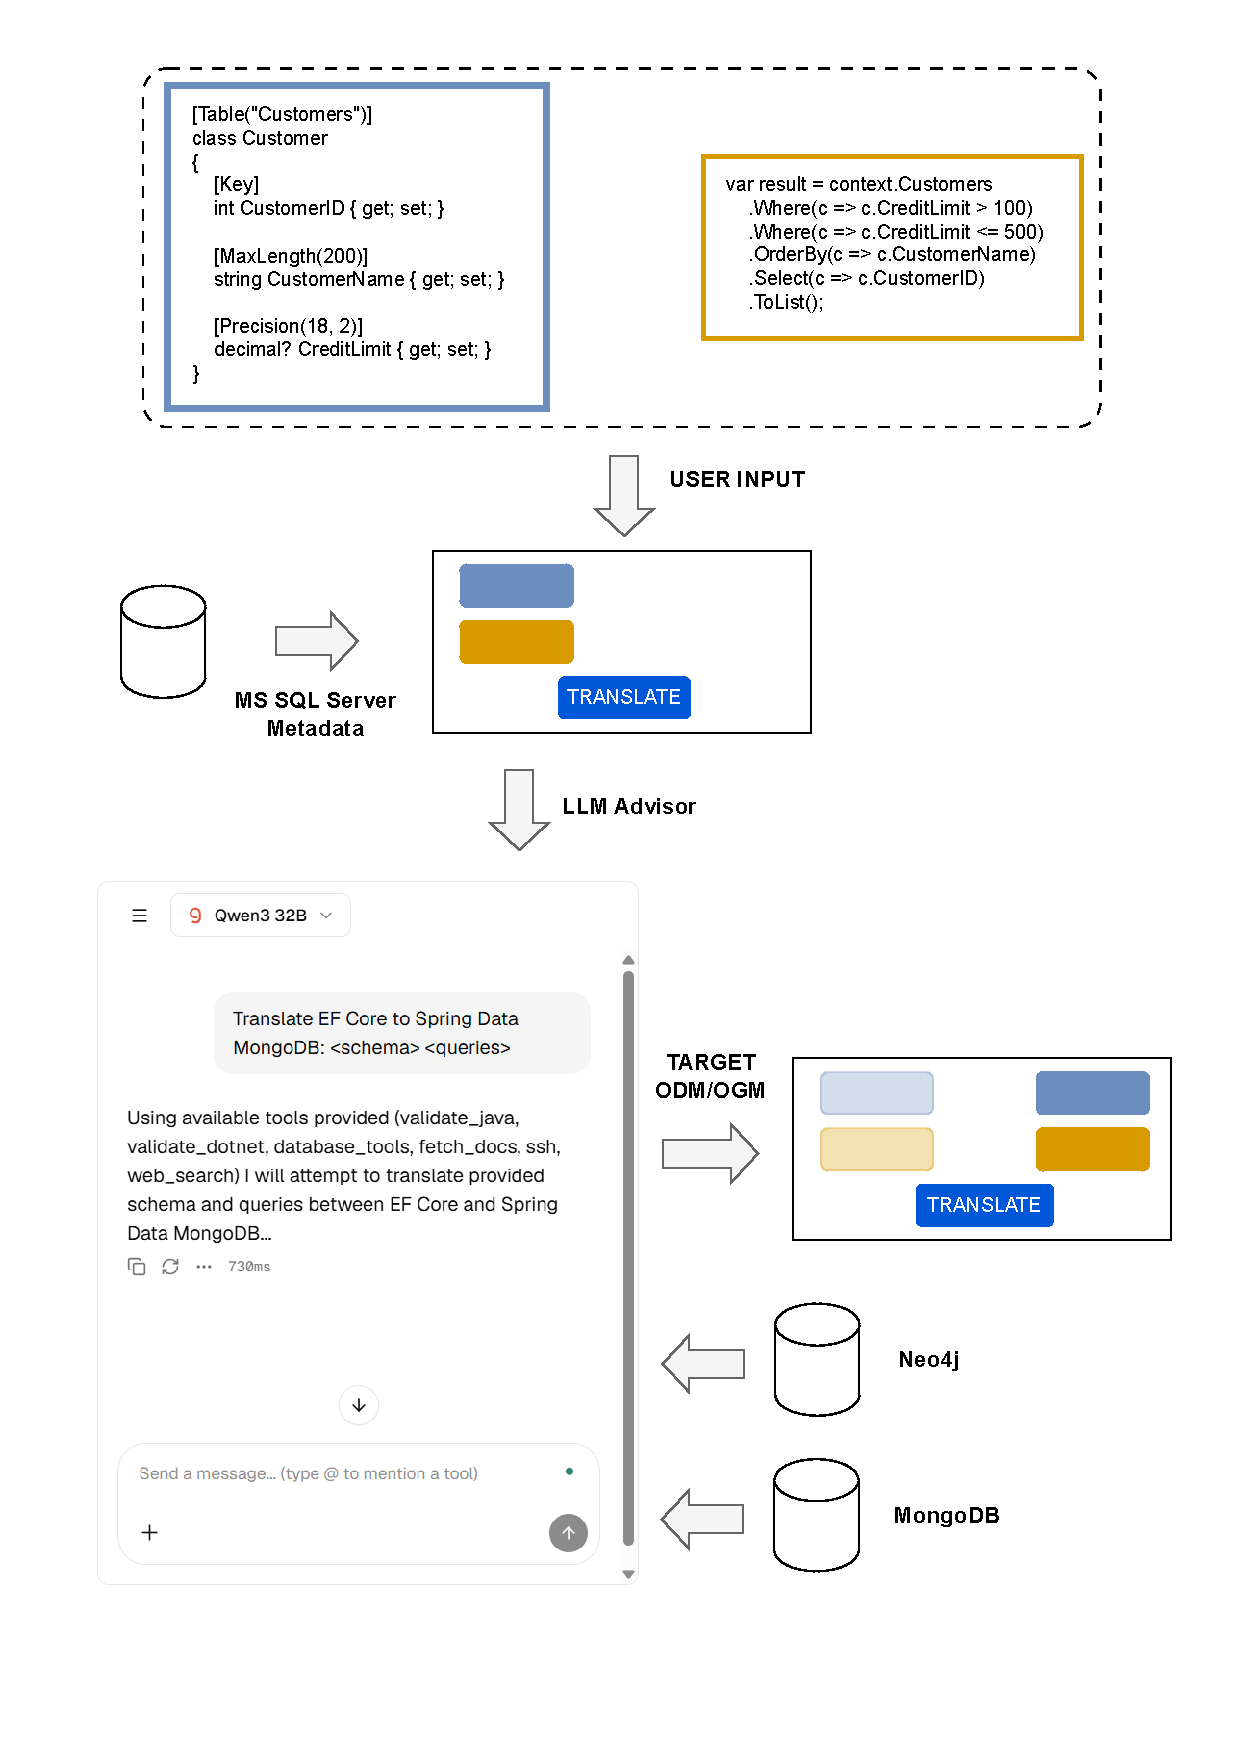
\includegraphics[width=\textwidth, height=0.85\textheight, keepaspectratio]{img/uom-workflow.pdf}
\caption{User interaction flow example after integration of the LLM Advisor. Before: User Input (EF Core entity + LINQ query) $\to$ Intermediate Representation (Entity/PropertyMap, QueryInstructions) $\to$ Target ORM code (Dapper SQL). After integration: User Input (EF Core entity + LINQ query) $\to$ LLM Advisor UI widget $\to$ LangGraph API Server $\to$ Target OGM/ODM code (e.g. Spring Data MongoDB).}
\label{fig:uom-workflow}
\end{figure}

The updated workflow (see Figure~\ref{fig:uom-workflow}) proceeds as follows:
\begin{enumerate}
  \item ORMorpher and MS SQL Server are initialized with a sample dataset using Docker.
  \item The user is asked to configure mapping for MongoDB in MongoDB Relational Migrator\footnote{\url{https://www.mongodb.com/products/tools/relational-migrator}}, and for Neo4j in Neo4j ETL Tool\footnote{\url{https://neo4j.com/labs/etl-tool/}}, and then the ETL pipelines are executed. This is a one-time semi-automatic setup to define how relational tables/columns map to document/graph structures.
  \item The user provides source-framework schema and queries via the ORMorpher UI and the LLM Advisor UI plugin.
  \item The \textbf{Orchestrator} extracts database schemas (MS SQL Server, MongoDB, Neo4j) to provide ground-truth schema context to the LLMs.
  \item The LangGraph \textbf{Translation Agent} iteratively generates and validates code using various tools (e.g. JavaCompiler class, or Maven CLI) in sandboxed Docker environments.
  \item Compilation/validation errors, query execution plans, query result schemas, etc. are fed back to the agent; it refines code up to a configurable retry limit. A manual user interaction is triggered if retries are exhausted.
  \item Results are displayed in the UI.
\end{enumerate}


\subsection{Functional Requirements}

\begin{itemize}
  \item \textbf{F01 ETL Pipeline:} Provide scripts or workflows to initialize and populate MS SQL Server, MongoDB, and Neo4j from a sample dataset.
  \item \textbf{F02 Schema Translation:} Given source entity classes for EF Core, NHibernate, or Dapper, produce equivalent (with respect to relational-document/graph mapping) entity classes for Spring Data MongoDB or Spring Data Neo4j.
  \item \textbf{F04 Query Translation:} Translate LINQ / Dapper-SQL queries from a source .NET ORM to logically (with respect to data model mapping) equivalent\footnote{Equivalent queries output logically same results but in different formats, e.g. CSV tables vs. JSON documents, but in context of ORM/ODM/OGM frameworks we should get similar instances (i.e. logically equivalent properties) of entities in supported languages (e.g. C\# objects vs. Java objects)} queries for target Java Spring Data frameworks.
  \item \textbf{F06 Iterative Refinement:} Translation workflow must iteratively correct errors based on compilation/validation feedback until code is valid or a retry/timeout limit is reached.
  \item \textbf{F07 Manual Intervention:} When the retry limit is exhausted, stop and present the current state to the user for manual correction.
  \item \textbf{F10 UI Plugin:} Integrate an LLM translation widget into the existing ORMorpher ASP.NET frontend; show translation logs, prompts, LLM outputs, and/or validation results.
  \item \textbf{F11 REST API:} Expose a LangGraph API Server REST API for external triggering of translations and retrieval of results.
  \item \textbf{F12 Configurable LLM Backend:} LLM providers (Ollama~\cite{ollama} server hosted by XRG at KSI MFF UK~\cite{xrg-mff}, CERIT-SC vLLM hosted by e-INFRA CZ (Metacentrum)~\cite{einfra}, or any other OpenAI-compatible API) must be swappable via environment configuration.
\end{itemize}

\subsection{Non-Functional Requirements}

\begin{itemize}
  \item \textbf{N01 Performance:} End-to-end translation should complete within a reasonable time frame (e.g. under 5 minutes for simple one-entity schema, and simple select queries).
  \item \textbf{N02 Observability:} All LLM calls, tool invocations, token counts, and retry chains must be traced via Observability tools (e.g. LangSmith\footnote{\url{https://docs.langchain.com/langsmith/home}}) for later analysis.
  \item \textbf{N03 Deployment:} The entire system must be containerized using Docker Compose (services include ORMorpher, databases, LangGraph ecosystem, translation tools, etc.).
  \item \textbf{N04 Security:} The system must be designed with security best practices in mind, especially when executing generated code in sandboxed environments. Proper isolation and resource limits must be enforced.
  \item \textbf{N05 Open Source:} Source code must be publicly available under an open-source licence on GitHub~\cite{uomrepo}.
\end{itemize}

\subsection{Mockups}

The primary user interface for the \emph{LLM Advisor} is an embedded UI widget integrated into the existing ORMorpher web application, as shown in Figure~\ref{fig:ui-mockup}. The interface is divided into two main parts:

\begin{itemize}
  \item \textbf{Background App (ORMorpher UI):} Allows users to select source frameworks, input source schemas (e.g., C\# classes) and queries (e.g., LINQ), and view legacy heuristic translations.
  \item \textbf{LLM Advisor Plugin:} A standalone modal assistant located in the lower right corner. Users can select target frameworks, trigger translations by sending custom prompts with source/target/code information (free form, or possibly through dropdowns), and trigger AI-driven translation workflows. Finally, it streams translated code natively into the assistant with optional error-handling/fallbacks and possible manual user input.
\end{itemize}

This plugin can optionally be integrated into other web applications or accessed programmatically via its REST API. The design remains subject to change as development progresses.

\begin{figure}[htb]
  \centering
  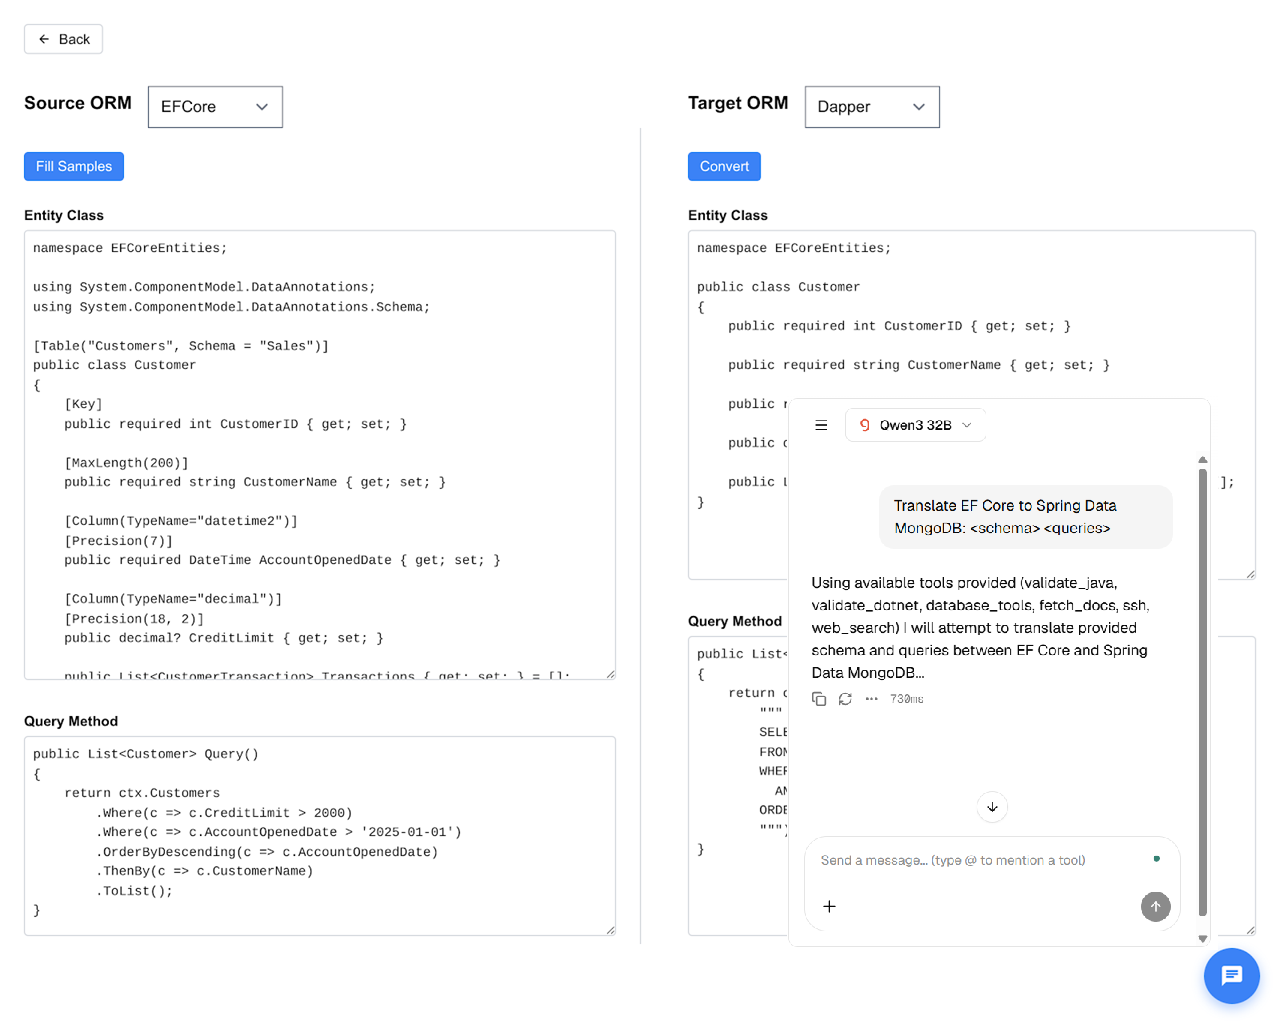
\includegraphics[width=0.95\textwidth]{img/ui-mockup.png}
  \caption{UI after integration of the LLM Orchestrator. From existing ORMorpher two-panel layout (Source/Target ORM dropdowns, Entity C\# class input, LINQ/Dapper-SQL Query inputs, Convert button, translated C\# code), to the same UI but with the LLM Advisor plugin.}
  \label{fig:ui-mockup}
\end{figure}

\subsection{Architecture}
\label{subsec:architecture}

The \emph{UOM} system uses Docker Compose for portable containerization. Its architecture, illustrated using C4 model diagrams (System Context Level 1 in Figure~\ref{fig:c4-level1} and Container Level 2 in Figure~\ref{fig:c4-level2}), consists of four primary components:

\begin{itemize}
  \item \textbf{ORMorpher Web UI:} The frontend interface capturing user inputs and displaying translated outputs via REST API or SSE.
  \item \textbf{LangGraph Orchestrator:} The core Python LLM engine managing workflow agents, tool coordination, and state persistence (PostgreSQL/Redis).
  \item \textbf{Validation Sandboxes:}\footnote{The sandbox services are initial proposals and may be refactored or replaced if more efficient, secure runtime evaluation alternatives are discovered during development.} Isolated execution environments (currently proposed as a .NET Service\footnote{This service may be represented by existing ORMorpher application alone, since the target translation frameworks don't include .NET ORMs. This functionality is already implemented in its original heuristic-based approach.} and Java Service) for verifying syntactic and functional code correctness through dynamic compilation (e.g., Roslyn/dotnet CLI, JavaCompiler/Maven).
  \item \textbf{Databases \& ETL:} Source/target data stores (MS SQL Server, MongoDB, Neo4j) and ETL tools (MongoDB Relational Migrator, Neo4j ETL Tools) ensuring schema and sample data availability for translations.
\end{itemize}



\begin{figure}[htb]
  \centering
  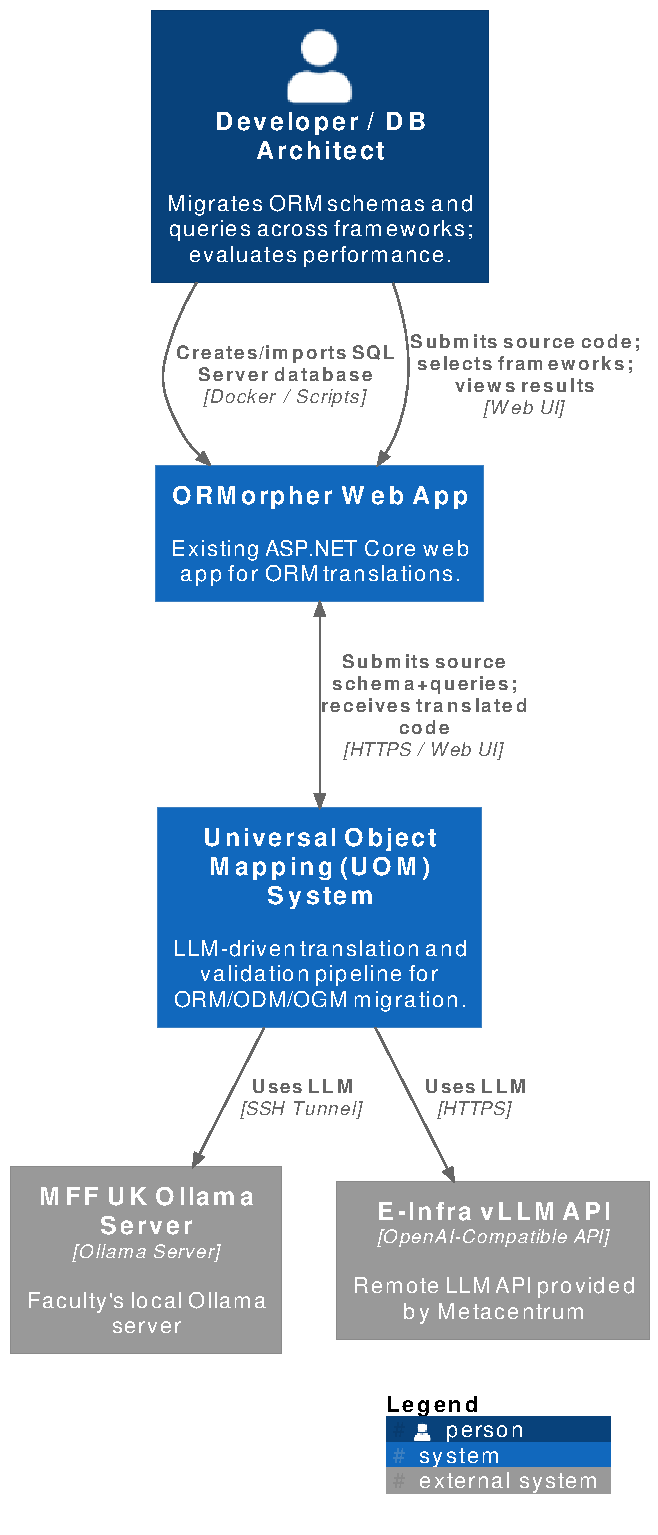
\includegraphics[scale=0.5]{img/uom-c4-architecture-level1.pdf}
  \caption{System Context (Level 1) diagram showing the Universal Object Mapping (UOM) system as a central component interacting with the user, the existing ORMorpher web app, and external LLM providers (Ollama server and E-infra vLLM API~\cite{einfra}).}
  \label{fig:c4-level1}
\end{figure}

\begin{figure}[htb]
  \centering
  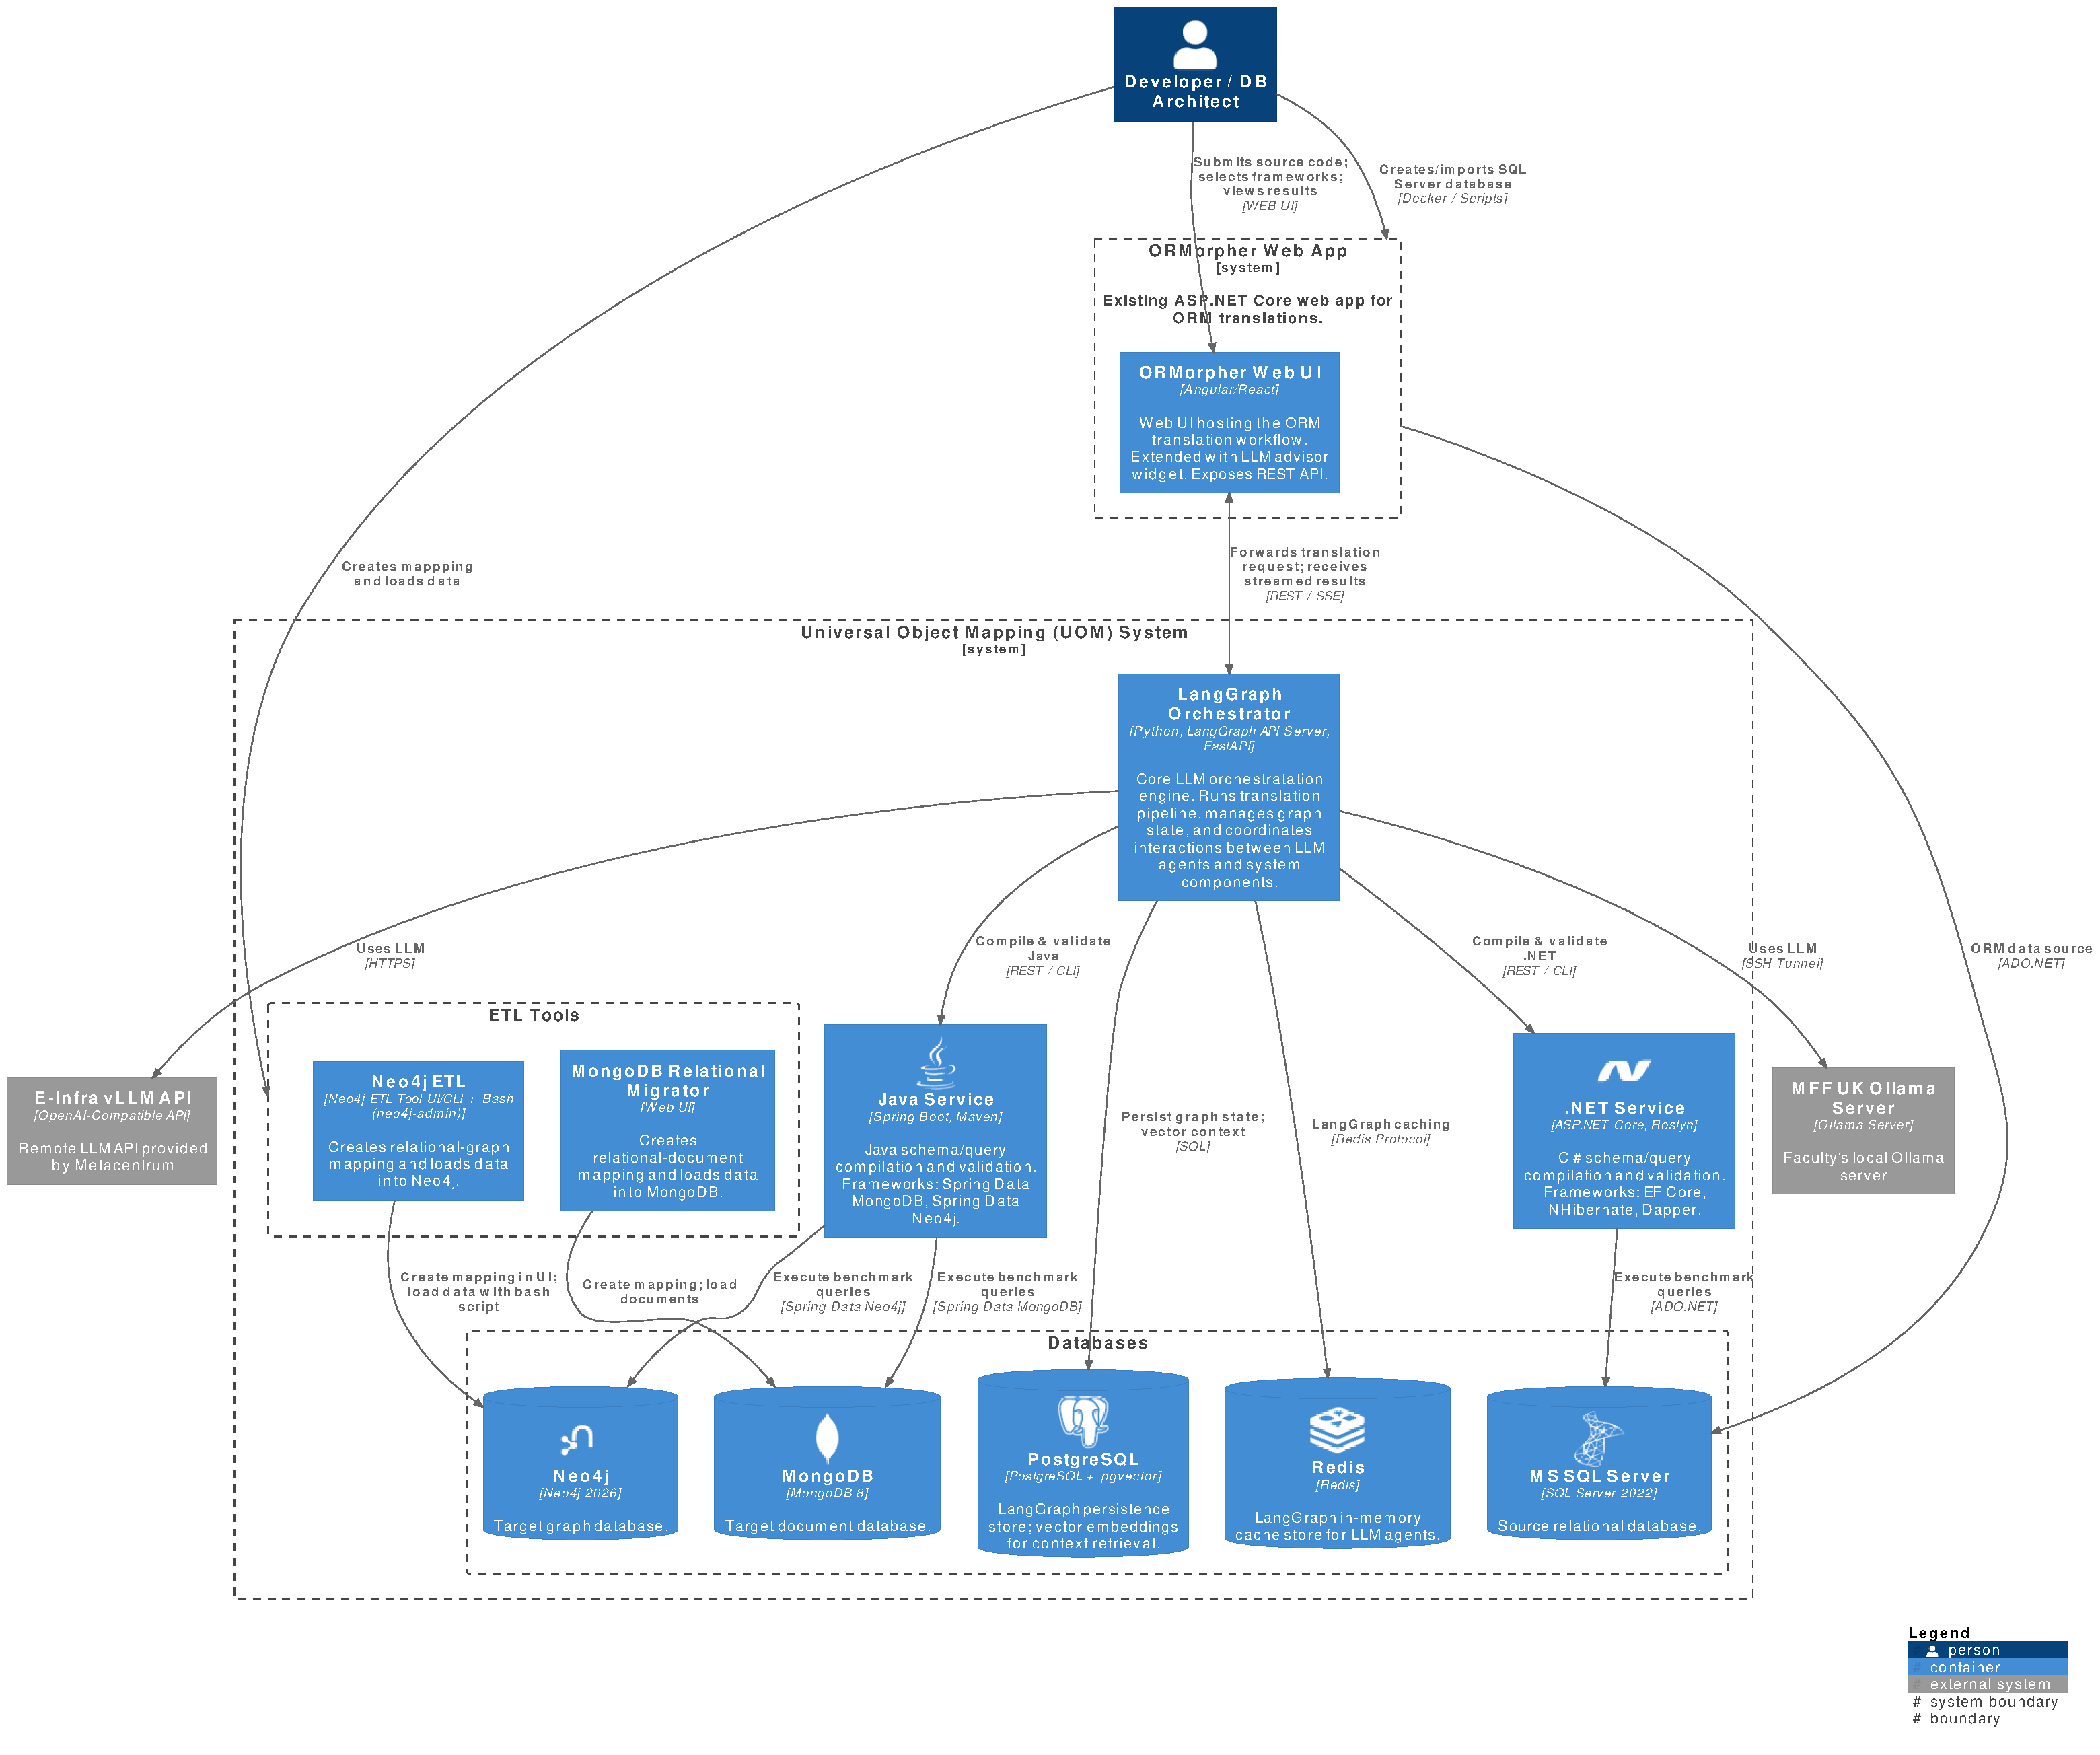
\includegraphics[scale=0.3]{img/uom-c4-architecture-level2.pdf}
  \caption{Container (Level 2) diagram showing the internal structure of the Universal Object Mapping (UOM) system, including the LangGraph (LLM) Orchestrator, validation services, databases, ETL Tools, and external LLM providers.}
  \label{fig:c4-level2}
\end{figure}

\section{Platform and Technologies}

The project relies on a diverse technology stack to handle the multi-language compilation, LLM orchestration, and data storage requirements. The chosen technologies are grouped as follows:

\begin{itemize}
  \item \textbf{Orchestrator:} Python, LangGraph API Server, LangChain, LangSmith (or other Observability platform), \texttt{uv}. Used to build the core AI orchestration layer, managing the stateful ReAct agents and their workflow.
  \item \textbf{LLM Providers:} MFF UK Ollama Server (e.g. \texttt{qwen3-coder:30b}), E-infra vLLM OpenAI-compatible API~\cite{einfra} (e.g. \texttt{kimi-k2.5}), any OpenAI-compatible endpoint. Provides the necessary reasoning capabilities, supporting both local inference and high-performance remote models.
  \item \textbf{.NET Service:} C\# / ASP.NET Core / .NET, Roslyn Scripting API, EF Core, NHibernate, Dapper. Provides a dedicated runtime environment for dynamically compiling, validating, and testing generated .NET framework code.\footnote{Possibly not implemented in favour of existing ORMorpher application. See note in Section \ref{subsec:architecture}.}
  \item \textbf{Java Service:} Java, Spring Boot, Spring Data Neo4j, Spring Data MongoDB, Maven. Acts as a standalone sandbox for validating and compiling target schema and query code for Java-based NoSQL frameworks.
  \item \textbf{Frontend:} ASP.NET Core, Angular / React, Node.js. Retains the existing ORMorpher stack to present a familiar user interface that integrates the new LLM Advisor plugin.
  \item \textbf{Databases:} MS SQL Server, MongoDB, Neo4j, PostgreSQL, Redis. Combines source relational and target NoSQL databases for benchmarking, supplemented by PostgreSQL and Redis for orchestrator state persistence and caching.
  \item \textbf{ETL:} Bash, MongoDB Relational Migrator, Neo4j ETL Tool + \texttt{neo4j-admin} CLI. Used to map and migrate relational schemas and sample datasets into NoSQL models prior to running translation pipeline.
  \item \textbf{Infrastructure:} Docker, Docker Compose. Containerizes all system components to ensure portability, isolated sandboxing for code execution, and streamlined configuration.
  \item \textbf{Dev OS:} Linux / Ubuntu 24.04+ or WSL2 on Windows; Windows for .NET. Ensures seamless compatibility with containerized environments and error-free development workflow.
\end{itemize}

\section{Evaluation}

For evaluation, we will choose a sample representative ORM schema and queries from the WideWorldImporters dataset\footnote{\url{https://learn.microsoft.com/en-us/sql/samples/wide-world-importers-what-is?view=sql-server-ver17}} (or some other relational dataset), covering various query types (simple selects, joins, aggregations). We will then run the translation pipeline for sample source-target framework pairs (EF Core $\to$ Spring Data MongoDB, EF Core $\to$ Spring Data Neo4j, NHibernate $\to$ Spring Data MongoDB, etc.). Afterwards, the evaluation of the results can be conducted along two dimensions: \emph{translation correctness} and \emph{LLM orchestrator metrics}, although the final realisation may differ depending on the observed data during experimentation. 

\textbf{Translation Correctness:} We will run the pipeline on example source schema/queries and compare generated output with expected target output. As a possible result, evaluation metrics (e.g. accuracy) can be computed from the fraction of translations that compile without errors and return results consistent with the source-framework baseline. 

\textbf{Orchestrator Metrics:} Using Observability platform, we will perform API tracing to obtain metrics, for example, token consumption, tool call counts, exception rates, or retry chain lengths. Optionally, statistical analysis of LLM Advisor performance can be performed using the obtained data points.

\section{Risks}

The following section outlines the principal risks associated with the project and presents potential mitigation strategies. These measures should be understood as indicative rather than mandatory in their entirety, as their actual application will depend on the specific issues that arise during the course of the project.

\begin{itemize}
  \item \textbf{LLM Output Quality:} Hallucinated code and framework APIs, knowledge caps, syntactically valid but semantically and logically wrong translations, weak models. 
  
  \emph{Mitigation:} multiple models used, iterative compilation feedback, manual inspection, validation, minimum model quality (Kimi K2.5 / GLM-5 class or better).
  \item \textbf{Context Explosion:} Long tool call histories may overflow LLM context windows.
  
  \emph{Mitigation:} multiple agents/nodes with separate contexts, LangGraph state summarization, configurable context pruning, retry limits.
  \item \textbf{Framework/Data Model Heterogeneity:} Structural mismatches (embedded documents vs.\ references, graph traversal vs.\ SQL joins) may prevent exact semantic equivalence. Data model differences may lead to subjectively non-equivalent translations. Mappings may be inefficient, e.g. translating each relational table to a separate document collection, which may lead to suboptimal queries, performance issues, and user dissatisfaction.
  
  \emph{Mitigation:} careful prompt engineering, iterative refinement, manual user intervention, giving more freedom to LLM (e.g., allowing to explain their reasoning, suggest improvements, etc.), and automatic heuristic-based mappings pre-configured by used ETL tools.
  \item \textbf{External Dependencies Maturity:} We will use external dependencies (e.g. MongoDB Relational Migrator, Neo4j ETL Tool) for the ETL process, relatively new MCP servers for agents (databases, docs, validation), CLI tools, Docker images, etc. which may have bugs or limitations. 
  
  \emph{Mitigation:} careful selection, early testing, fallbacks, and clear documentation of used dependencies and their known limitations.
  \item \textbf{LLM Provider Availability:} Remote LLM services may have rate limits or downtime. 
  
  \emph{Mitigation:} two default LLM providers configured, with custom configurable OpenAI-compatible endpoint option.
  \item \textbf{Security:} Executing generated code in sandboxed environments poses security risks. 
  
  \emph{Mitigation:} strict resource limits, isolation, and monitoring of execution environments.
\end{itemize}

\section{Milestones / Deliverables}

\begin{itemize}
  \item \textbf{D1 --- Architecture \& Design:} Design Docker Compose stack, networking, automation using scripts, design ETL processes -- all three databases initialized (MS SQL Server, MongoDB, Neo4j) with WideWorldImporters dataset in different data models with sample mappings.
  \item \textbf{D2 --- Core Translation Pipeline:} LangGraph graph (extracting input, translation, validation) operational, including LLM providers, relevant tools/MCP servers, and external dependencies integrated.
  \item \textbf{D4 --- UI Plugin:} LLM Advisor UI widget for translation between ORM/ODM/OGM frameworks.
  \item \textbf{D3 --- Full E2E Pipeline:} User interaction flow: ETL, UI plugin interaction (setup, input), sample ORM $\rightarrow$ ODM/OGM translation, Advisor UI output. At least one end-to-end translation (EF Core $\to$ Spring Data Neo4j) verified by testing.
  \item \textbf{D5 --- Evaluation:} Correctness metrics for sample framework pairs, observable LangGraph trace analysis, and potential conference demo paper.
  \item \textbf{D6 --- Documentation:} User and programmer documentation, setup guide.
\end{itemize}

A live demo will be presented during defense using local development setup. Source code will be available at \url{https://github.com/corovcam/Universal-Object-Mapping}.

\section{Time Schedule}

Although the project timeline is intentionally structured in weeks rather than months, the overall effort is estimated at approximately 320 hours (around 40 person-days). The work is being pursued in parallel with the solver’s diploma thesis, with the project concentrating mainly on the software implementation and experimental realization, while the diploma thesis addresses the associated theoretical foundations, methodology, and scholarly interpretation of the results. The Table \ref{tab:time-shedule} below presents the detailed milestones and time schedule.

\begin{table}[H]
\centering
\begin{tabular}{ | m{10em} | m{23em} | m{3.5cm} | m{1.3cm} | }
\hline
Milestone & Activity & Time schedule & Man-days \\
\hline
D1: Architecture \& Design & Design databases, Docker Compose, ETL, UI & Week 1--2 & 4 \\
              & Infrastructure setup, initialization, refinement & Weeks 1--2 & 3 \\
\hline
D2: Core Translation Pipeline & Graph design, tools selection, initial setup & Weeks 2--3 & 4 \\
              & Graph setup, LLM/tools integration, testing & Weeks 3--5 & 9 \\
\hline
D3: UI Plugin & UI package development & Weeks 5--6 & 4 \\
              & Integration & Weeks 5--6 & 2 \\
\hline
D4: Full E2E Pipeline & Implement and polish full end-to-end user interaction flow & Weeks 6--8 & 8 \\
\hline
D5: Evaluation & Correctness evaluation, tracing analysis & Weeks 8--9 & 4 \\
\hline
D6: Documentation & User/programmer docs, deployment notes & Week 9 & 2 \\
\hline
\end{tabular}
\label{tab:time-shedule}
\end{table}

\section{Form of Collaboration}

The project will be supervised by \textit{Pavel Koupil}, with whom the solver will regularly discuss the research framing, methodological choices, overall conceptualization of the proposed solution, and the formulation of outputs. He will also provide continuous feedback on the technical direction of the project, the evaluation design, and the interpretation of the obtained results. Close collaboration is also planned with \textit{Irena Holubová}, who will provide strategic oversight and ensure alignment of the project with the broader research agenda of the Adaptive Data Management Research Group (ADaM). In addition, other experts from the ADaM research group will contribute domain-specific consultation as needed, particularly in areas related to multi-model data management, framework interoperability, and the design of the translation pipeline.

\textit{Martin Čorovčák}, as the solver, will be fully responsible for the implementation of the proposed solution and will also take primary responsibility for its practical realization, including integration, experimentation, and technical validation.

\subsection{Consulting Plan}

An initial meeting with \textit{Pavel Koupil} and \textit{Irena Holubová} has already taken place to define the project scope, clarify its objectives, and establish the overall collaboration framework. These discussions focused on the intended research direction, expected outcomes, and the broader positioning of the project within the ADaM research agenda.

Following this, regular meetings with \textit{Pavel Koupil} will be held to monitor progress, discuss encountered challenges, refine the methodological and technical direction, and determine the next steps in the project. These meetings will also serve as a space for continuous feedback on implementation decisions, evaluation design, and the interpretation of intermediate results.

Most meetings will take place either in person at the faculty building or online, depending on current needs and availability. They are expected to be held approximately once or twice a week and to last around sixty minutes. In addition, ad-hoc consultations will be arranged whenever necessary to address specific technical issues, discuss partial outputs, or obtain timely feedback on important decisions.


\subsection{Collaboration with Other Team Members}

The solver will cooperate with several experts whose knowledge covers the main research dimensions of the project. In the area of relational databases, data modeling, and query processing, the primary consultations will be conducted with \textit{Pavel Koupil} and \textit{Irena Holubová}. Their expertise will be particularly relevant for issues related to schema interpretation, preservation of query semantics, and the database foundations of migration between mapping frameworks. Where appropriate, additional consultation may also be provided by \textit{Michal Kopecký} on selected database-related topics.
In the area of LLMs, NLP, and AI, the solver may consult researchers such as \textit{Roman Barták}, particularly with regard to the design of the LLM-based translation process, prompting strategies, agent reasoning, and validation of generated outputs. Such consultations will support the methodological quality of the proposed approach and help align it with current developments in AI-assisted software engineering.
Additional feedback may also be obtained from software engineering and database colleagues within the Adaptive Data Management Research Group (ADaM), especially in matters concerning implementation, integration, and evaluation. This collaborative background will contribute to both the quality of the resulting solution and its consistency with the broader research agenda of the group.

\begin{thebibliography}{99}

\bibitem{mmcat}
KOUPIL, Pavel, SVOBODA, Martin and HOLUBOVÁ, Irena, 2021. MM-cat: A Tool for Modeling and Transformation of Multi-Model Data using Category Theory. In: 2021 ACM/IEEE International Conference on Model Driven Engineering Languages and Systems Companion (MODELS-C). Online. October 2021. p.635–639. DOI 10.1109/MODELS-C53483.2021.00098. Available from: \url{https://doi.org/10.1109/MODELS-C53483.2021.00098} [Accessed 1 April 2026]. 

\bibitem{ormorpherthesis}
ABRAHÁM, Milan, 2025. Framework-Agnostic Query Adaptation: Ensuring SQL Compatibility Across .NET Database Frameworks. Online. 9 September 2025. Available from: \url{https://dspace.cuni.cz/handle/20.500.11956/203083} [Accessed 31 March 2026].

\bibitem{ormorpherrepo}
ORMConvertor repository. GitHub. Online. Available from: \url{https://github.com/milan252525/orm-convertor/tree/main/ORMConvertor} [Accessed 31 March 2026].

\bibitem{ase2025}
ABRAHÁM, Milan and KOUPIL, Pavel, 2026. ORMorpher: An Interactive Framework for ORM Translation and Optimization. In: 2025 40th IEEE/ACM International Conference on Automated Software Engineering (ASE). Online. Seoul, Korea, Republic of: IEEE Press. 28 January 2026. p. 4037–4040. DOI 10.1109/ASE63991.2025.00369. Available from: \url{https://doi.org/10.1109/ASE63991.2025.00369} [Accessed 31 March 2026].

\bibitem{uomrepo}
ČOROVČÁK, Martin, 2026. Universal Object Mapping repository [software]. Online. 8 March 2026. Available from: \url{https://github.com/corovcam/Universal-Object-Mapping} [Accessed 31 March 2026].

\bibitem{xrg-mff}
XRG - XML and Web Engineering Research Group at KSI MFF UK. Online. Available from: \url{https://xrg.cz/} [Accessed 1 April 2026].

\bibitem{ollama}
Ollama [software]. Online. 1 April 2026. Ollama. Available from: \url{https://github.com/ollama/ollama} [Accessed 1 April 2026].


\bibitem{einfra}
e-INFRA CZ AIaaS Documentation. Online. Available from: \url{https://docs.cerit.io/en/docs/ai-as-a-service/introduction} [Accessed 31 March 2026]. 

\end{thebibliography}

\end{document}
